\documentclass[5p,times]{elsarticle}
% Draft in Elsevier's generic two-column layout. Page limit, highlights and front matter follow the
% target journal's Guide for Authors once it has been read (docs/PAPER_OUTLINE.md).
% Every number is taken from results/paper_numbers.json (unrounded values and bound-safe ranges).

\usepackage{amsmath,amssymb}
\usepackage{booktabs}
\usepackage{graphicx}
\usepackage{url}
\usepackage[hidelinks]{hyperref}
\usepackage{microtype}
\emergencystretch=1.5em

\journal{Pattern Recognition Letters}

\newcommand{\SA}{\mathrm{SA}}
\newcommand{\gtt}{\mathrm{GT}_{\mathrm{true}}}

\begin{document}

\begin{frontmatter}

\title{How much does a tracker-seeded ground truth favour its seed?\\
Measuring seed bias in multi-object tracking benchmarks}

% Author list, affiliations and e-mails to be confirmed by the authors.
\author[uef]{Trong Nghia Le}
\author[uef]{Thien Bao Nguyen\corref{cor}}
\cortext[cor]{Corresponding author.}
\affiliation[uef]{organization={3ITech, College of Technology and Design, University of Economics Ho Chi Minh City (UEH)},
  city={Ho Chi Minh City}, country={Vietnam}}

\begin{abstract}
Ground truth for multi-object tracking is increasingly produced by correcting a tracker's output. If the
same ground truth is used for evaluation, every error the reviewer leaves in place favours the seed
tracker. We measure this seed bias. A parametric reviewer model turns a seed tracker's output and the
complete public ground truth of MOT17, DanceTrack and the traffic benchmark FastTrack into simulated
reviewed ground truth. With four trackers on a shared detector and an assumed reference reviewer, the
seed's advantage over the other trackers is 0.069, 0.160 and 0.049 IDF1, with 95\% lower bounds far above
a pre-specified relevance threshold of 0.01. Around this reviewer the advantage grows almost linearly
with the share of identity errors left unfixed, by 0.006--0.033 IDF1 per tenth, and an external
appearance-based seed gives a similar advantage. Seed-correlated errors reorder the other trackers more
than random errors of the same number and size. Seeding from the union of several trackers helps little
and favours its members; consensus seeding reduces the distortion but does not protect trackers outside
the consensus; and a bracket over single-seed ground truths never contained the true score. Code and protocol are released.
\end{abstract}

\begin{keyword}
multi-object tracking \sep benchmark \sep ground truth \sep annotation bias \sep evaluation
\end{keyword}

\end{frontmatter}

\section{Introduction}
\label{sec:intro}

Annotating identities for multi-object tracking (MOT) frame by frame is expensive, so ground truth (GT)
is increasingly produced by running a tracker, or a detector with propagation, and asking people to
correct the result \cite{hao2023divotrack,voigtlaender2019mots,ravi2024sam2,nae2026indoorcrowd,fang2025calves}.
The procedure is efficient, and tracker-generated labels have been shown to train trackers well at a
fraction of the annotation cost \cite{cetintas2024spam}. When the corrected output is also used to
\emph{evaluate} trackers, however, every error that the reviewer leaves in place is an error that the
seed tracker shares, and the seed is rewarded for it. In at least one recent benchmark the seeding
tracker is also among the evaluated baselines \cite{nae2026indoorcrowd}.

The mechanism is known elsewhere. In dependency parsing, gold standards produced by correcting parser
output raise the seeding parser's labelled attachment score by 5.8--6.9 points relative to human-annotated
gold, and its lead over another parser by 3.6--4.1 points \cite{berzak2016anchoring}. In machine
translation, references post-edited from a system's output are by design closest to that system
\cite{snover2006hter}, and post-edits of several systems are used as joint references to reduce this
dependence \cite{bentivogli2018pe}. Quality-assessment tools for diagnostic accuracy studies check whether
the index test formed part of the reference standard (incorporation bias) and whether the reference was
read with knowledge of the index test \cite{whiting2003quadas,whiting2011quadas2}. In tracking and video
segmentation, dataset authors have noted that GT pre-generated by a model favours that model: DIVOTrack
restricted labels to objects with more than 30\% visibility and reviewed the whole dataset after
interpolation \cite{hao2023divotrack}, and SA-V annotated its evaluation splits without the video model in
the loop \cite{ravi2024sam2}. Neither study measured the effect, its dependence on how careful the reviewer
is, or whether such precautions remove it, and we are not aware of any study that does so for MOT.

We ask three questions. (RQ1) How large is the advantage a seed tracker gains on GT built from its own
output? (RQ2) Do seed-correlated GT errors reorder trackers more than random errors of the same number and
size? (RQ3) Do inexpensive annotation protocols reduce the bias? We answer them by simulation on public
benchmarks whose complete GT serves as the reference, with a reviewer model whose parameters can be read
as properties of an annotation process, and under a protocol fixed in version control before any
experiment. Our contributions are: (i) a measurement of seed bias in MOT on three benchmarks, which at an
assumed reference reviewer is larger than most differences between the evaluated trackers; (ii) the
descriptive finding that, around that reviewer, the advantage depends mainly on how many identity errors
are fixed, almost linearly, while box geometry contributes nothing; (iii) evidence that seed-correlated
errors distort the ranking of the \emph{other} trackers more than random errors; and (iv) an evaluation of
union seeding, consensus seeding and bracketing, including negative results.

\section{Related work}
\label{sec:related}

\textbf{Ground-truth quality and rankings.} Milan et al.\ showed that alternative annotations of the same
sequences change tracker rankings \cite{milan2013challenges}; their annotations differ independently of
the trackers, whereas seeded GT differs in the direction of one of them. Test-set label errors are common
in classification and can reorder models \cite{northcutt2021pervasive}. Re-annotating COCO masks with a
model-assisted pipeline flips the ranking of several detector pairs, mostly in favour of models that
predict sharper masks \cite{singh2024cocorem}, while a re-annotation of four detection benchmarks finds
missing objects to be the dominant error and reports that scores are highly sensitive to annotation
quality while rankings remain largely stable \cite{penquitt2026incomplete}. These studies treat label
errors as properties of the dataset rather than of an evaluated model.

\textbf{Assisted annotation in tracking.} Video annotation tools reduce cost by interpolating or
propagating sparse human input \cite{vondrick2013vatic,manen2017pathtrack}; model-in-the-loop engines let a
model propose whole tracks or masks for correction \cite{voigtlaender2019mots,ravi2024sam2}. TETA evaluates
trackers under incomplete annotation \cite{li2022teta}, and SPAM trains trackers on tracker-generated
labels with targeted human effort \cite{cetintas2024spam}. None of these analyses what happens when
assisted labels are the reference for evaluation.

\textbf{Pre-annotation bias.} Pre-annotation speeds up annotation; dictionary pre-annotation of clinical
entities showed no detectable bias \cite{lingren2014preannotation}, whereas correcting parser output
anchored treebank annotation toward the parser \cite{berzak2016anchoring}, and post-edited references in
machine translation are known to favour the edited system \cite{snover2006hter,bentivogli2018pe}.

\section{Seeded ground truth and the reviewer model}
\label{sec:model}

Let $\gtt$ be the reference GT and $A$ a seed tracker. A reviewer with parameters
$\theta = (r, p_{fp}, q, a)$ edits the output of $A$ into simulated reviewed GT $\mathrm{GT}_A(\theta)$:
\begin{itemize}
\item seed boxes are matched to $\gtt$ frame by frame (Hungarian assignment over pairs with IoU $\ge 0.5$);
\item each run of consecutive missed GT boxes of one object is added with probability $r$;
\item each run of consecutive unmatched seed boxes of one seed identity is kept with probability $p_{fp}$;
an added GT box replaces an overlapping (IoU $\ge 0.1$) unmatched seed box;
\item seed identities are matched one-to-one to GT identities as in IDF1; a (seed id, GT id) pair outside
this matching is an identity error, and errors whose corrections interact (e.g. the two halves of a swap)
form one \emph{episode}, fixed with probability $q$ regardless of its length;
\item a matched box keeps the seed geometry with probability $a$.
\end{itemize}
With $(r, p_{fp}, q, a) = (1, 0, 1, 0)$ the reviewer reproduces $\gtt$; with $(0, 1, 0, 1)$ it returns the
seed output unchanged. The reviewer introduces no errors of its own.

For a metric $M$ (IDF1 unless stated), the \emph{self-seed advantage} of $A$ over another tracker $B$ is
\begin{equation}
\begin{split}
\SA(A,B) = {} & \bigl[M(A;\mathrm{GT}_A) - M(B;\mathrm{GT}_A)\bigr] \\
 & - \bigl[M(A;\gtt) - M(B;\gtt)\bigr],
\end{split}
\end{equation}
the change in $A$'s lead over $B$ caused by seeding. Because the reviewer only moves GT toward the seed,
$\SA$ is non-negative in expectation; individual pairs can be slightly negative (the smallest pairwise
value over all settings is $-0.023$). Its sign is therefore not evidence; the empirical content is its
magnitude, and we test $\SA \ge \delta$ with a minimal-relevance threshold $\delta = 0.01$ IDF1.

\section{Experimental setup}
\label{sec:setup}

\textbf{Data.} We use the public GT of MOT17 (seven training sequences) \cite{milan2016mot16,dendorfer2021motchallenge},
DanceTrack (25 validation sequences) \cite{sun2022dancetrack} and FastTrack (12 urban traffic CCTV videos,
nine classes) \cite{hashempoor2025fasttracker}. MOT17 GT was annotated from scratch \cite{milan2016mot16};
DanceTrack GT was annotated with frame-to-frame box propagation that annotators refined
\cite{sun2022dancetrack}, a seed shared by none of the evaluated trackers; FastTrack does not document its
annotation procedure. FastTrack classes are mapped to six evaluation classes (person, bus, truck, car,
bicycle, motorbike); tracker boxes centred in an ignore region are discarded unless they match a GT box of
the evaluated class. MOT17 follows TrackEval's preprocessing.

\textbf{Trackers.} Detections come from COCO-pretrained YOLO11x and YOLO11n \cite{ultralytics2024yolo11}
(input 1280\,px, confidence $\ge 0.05$). SORT \cite{bewley2016sort}, ByteTrack \cite{zhang2022bytetrack},
OC-SORT \cite{cao2023ocsort} and BoT-SORT without camera-motion compensation \cite{aharon2022botsort} run
with library defaults \cite{roboflow2025trackers}. ByteTrack, OC-SORT and BoT-SORT receive every detection
and apply their own thresholds; SORT, which has no low-score stage, receives detections with confidence
$\ge 0.25$, its activation threshold. Four trackers on two detectors give eight systems; the four YOLO11x
systems are the seeds. No detector or tracker was trained on any evaluation sequence, so absolute scores
are below leaderboard values. All trackers pass detector boxes through, so systems sharing a detector
output identical boxes for the detections they keep.

\textbf{Reviewer settings.} The reference reviewer $\theta_{ref} = (0.75, 0.1, 0.5, 1)$ is an assumption,
not a measurement; results are also reported, descriptively, over a grid of 192 settings
($r \in \{0, .25, .5, .75, .9, 1\}$, $p_{fp} \in \{0, .1, .25, .5\}$, $q \in \{0, .5, .9, 1\}$,
$a \in \{0, 1\}$) with ten random draws each and common random numbers across settings.

\textbf{Statistics.} IDF1 is pooled over all (sequence, class) units of a benchmark. Secondary metrics are
computed with TrackEval \cite{luiten2020trackeval}; IDF1 on simulated GT uses an exact reimplementation of
its Identity metric, checked against TrackEval in our tests. Intervals are 95\% BCa \cite{efron1987bca} over
10,000 bootstrap resamples of sequences with jackknife acceleration; MOT17 has seven sequences, so its
intervals are approximate. Confirmatory statements are made only at $\theta_{ref}$ and per benchmark; a
general statement requires all three benchmarks to pass. Variation between reviewer draws (standard
deviation 0.001--0.005 at $\theta_{ref}$) is small compared with variation between sequences.

\textbf{Protocol and deviations.} Hypotheses, the grid, the analyses and a stopping rule were fixed in
version control before any experiment; the protocol, its eight dated amendments and the commit history
are released. The amendments made before any result restated RQ1 as a magnitude test, replaced the RQ3
endpoint by the paired distortion difference below, and added a second detector in place of the planned
appearance-based tracker, which was not run. A planned study of real reviewers was deferred. Union seeding
was first dropped on an argument that the data later contradicted and was then run, after the other
results were known; its definition did not change. Analyses marked \emph{exploratory} were added after
the results.

\section{Results}
\label{sec:results}

\subsection{RQ1: size of the self-seed advantage}

\begin{table}[t]
\centering
\caption{Self-seed advantage at $\theta_{ref}$ (IDF1; mean over the 12 ordered pairs of YOLO11x systems
and ten draws), BCa 95\% intervals over sequences. LOO: range of leave-one-sequence-out estimates.
Cross-detector: seed (YOLO11x) against the YOLO11n systems. True-GT spread: range of the four YOLO11x
systems' IDF1 on $\gtt$.}
\label{tab:h1}
\small
\setlength{\tabcolsep}{1.6pt}
\begin{tabular}{@{}lccc@{}}
\toprule
 & MOT17 & DanceTrack & FastTrack \\
\midrule
Sequences & 7 & 25 & 12 \\
$\SA$ & 0.069 & 0.160 & 0.049 \\
BCa 95\% & [0.060, 0.089] & [0.148, 0.170] & [0.042, 0.059] \\
LOO range & [0.063, 0.074] & [0.158, 0.163] & [0.046, 0.051] \\
Cross-detector & 0.069 & 0.158 & 0.049 \\
\quad BCa 95\% & [0.058, 0.091] & [0.144, 0.170] & [0.041, 0.058] \\
Without SORT pairs & 0.061 & 0.145 & 0.039 \\
True-GT spread & 0.473--0.536 & 0.352--0.472 & 0.530--0.623 \\
\bottomrule
\end{tabular}
\end{table}

Table~\ref{tab:h1} reports the advantage. On every benchmark the lower confidence bound exceeds
$\delta = 0.01$ several times over, so the confirmatory hypothesis holds on all three. At $\theta_{ref}$
the advantage exceeds every pairwise IDF1 difference between the YOLO11x systems on MOT17 and DanceTrack
and half of them on FastTrack. It is largest on DanceTrack, where the seeds make the most identity errors,
consistent with its uniform appearance and diverse motion. It does not hinge on one tracker: without pairs
involving SORT it is 0.038--0.146, and with SORT fed every detection 0.058--0.173. Changing the matching
threshold of the reviewer from 0.5 to 0.4 or 0.6 changes it by at most 0.01. With car, bus and truck merged
into one FastTrack class it is 0.047 [0.038, 0.060]; removing the two FastTrack classes with more than
10\% class confusion leaves 0.050 [0.042, 0.060]; per class it ranges over 0.021--0.080. On secondary
metrics the advantage is 0.042--0.141 in HOTA$_{0.5}$ and is concentrated in association accuracy
(AssA$_{0.5}$: 0.059--0.196) rather than detection accuracy (DetA$_{0.5}$: 0.024--0.031).

\begin{figure*}[!t]
\centering
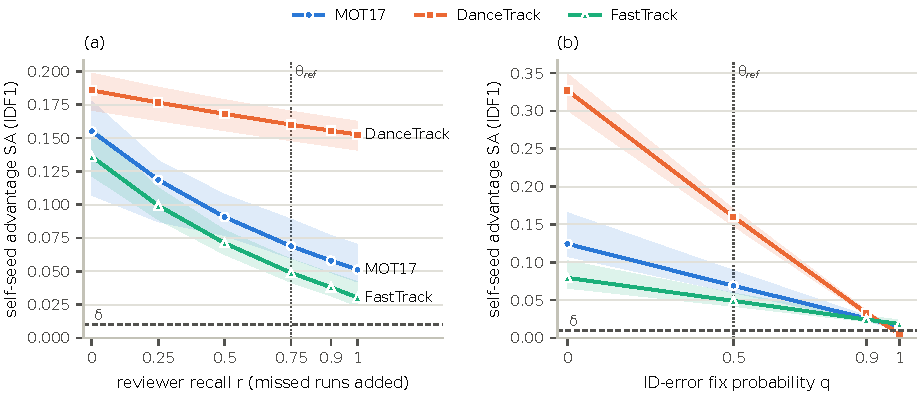
\includegraphics[width=\textwidth]{figures/fig_sa_curves.pdf}
\caption{Self-seed advantage as one reviewer parameter varies with the others at $\theta_{ref}$
(descriptive; shaded: pointwise BCa 95\%). (a) Recall of missed objects $r$. (b) Probability $q$ of fixing
an identity-error episode. The dashed line is $\delta = 0.01$.}
\label{fig:curves}
\end{figure*}

\textbf{Reviewer parameters (descriptive).} Fig.~\ref{fig:curves} varies one parameter at a time. Around
$\theta_{ref}$ fixing identity errors has the largest effect: fixing every episode ($q = 1$) leaves
0.015, 0.005 and 0.018 (MOT17, DanceTrack, FastTrack), still above $\delta$ on MOT17 and FastTrack, while
adding every missed object ($r = 1$) leaves 0.030--0.153. Over the whole range of $r$, however, missed
objects matter as much as identity on MOT17 and FastTrack. The advantage is close to linear in $q$
(linear interpolation between $q = 0$ and $q = 1$ is within 0.001 of the simulated value on MOT17 and
FastTrack and within 0.007 on DanceTrack): each tenth of episodes left unfixed adds 0.006--0.033 IDF1, so a
benchmark builder who measures $q$ on an audited sample can read off the expected advantage. In all 96
settings with $q \le 0.5$ the lower bound exceeds $\delta$ on every benchmark. The retention of false
positives changes the advantage by at most 0.013 over $p_{fp} \in [0, 0.5]$. Box geometry does not
contribute: with a shared detector it cannot, and against the other detector, where it can, replacing the
seed's geometry by the GT geometry changes the advantage by at most 0.005.

\textbf{An external seed (exploratory).} To check that the advantage is not specific to weak,
motion-based seeds, we used MPNTrack \cite{braso2019mpntrack}, a graph-based tracker with appearance cues
and its own detections, as the seed on MOT17, using its training-set outputs distributed with TrackEval.
MPNTrack was trained on these sequences (true IDF1 0.713), so it is a low-error seed and is not ranked. Its
advantage over our eight systems is 0.041 [0.024, 0.062] at $\theta_{ref}$, 0.082 at $q = 0$ and 0.004
[$-$0.004, 0.015] at $q = 1$.

\subsection{RQ2: ranking distortion}

\begin{figure}[!t]
\centering
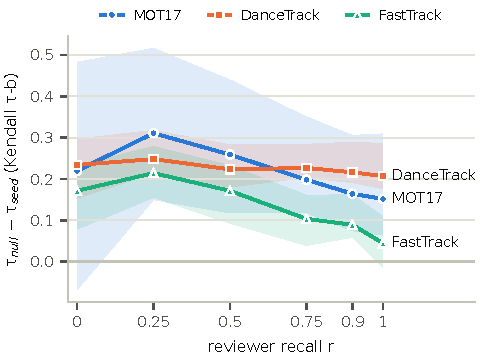
\includegraphics[width=\columnwidth]{figures/fig_h2.pdf}
\caption{Ranking distortion of seed-correlated errors relative to random errors of the same number and
length, as reviewer recall $r$ varies with the other parameters at $\theta_{ref}$ and GT geometry on both
sides ($a = 0$): $\tau_{null} - \tau_{seed}$ (Kendall $\tau$-b between rankings of eight systems on
simulated and true GT). $r = 0.75$ is the confirmatory point; shaded: pointwise BCa 95\%.}
\label{fig:h2}
\end{figure}

On seeded GT at $\theta_{ref}$, on average 3.2 (MOT17), 3.5 (DanceTrack) and 1.0 (FastTrack) pairs of
systems whose true IDF1 differs by more than $\delta$ are reversed. To separate the effect of correlation with
the seed from the effect of having errors at all, each seeded GT is paired with a null GT that requests the
same number and lengths of missed runs, unfixed identity errors and kept false-positive runs, placed at
random on the true GT, with GT geometry on both sides. Seed-correlated errors reduce rank agreement more:
$\tau_{null} - \tau_{seed}$ is 0.198 [0.118, 0.350], 0.227 [0.204, 0.284] and 0.104 [0.039, 0.161], and they
cause 2.35 [1.02, 4.08], 3.17 [2.98, 3.97] and 1.05 [0.28, 2.00] more reversals (Fig.~\ref{fig:h2}; the
interval includes 0 only at $r = 0$ on MOT17 and $r = 1$ on FastTrack). The null could not place 12\%
(DanceTrack) and 14\% (FastTrack) of the requested false-positive boxes, and 25--50\% of the kept
false-positive boxes in seeded GT carry the label of a real track, an error the null does not reproduce;
the endpoint is therefore approximate on DanceTrack and FastTrack, and the null is somewhat milder than
the seeded GT.

\textbf{Beyond the seed (exploratory).} The distortion is not only the seed moving up. Ranking the seven
systems other than the seed, seeded GT still agrees less with the truth than null GT:
$\tau_{null} - \tau_{seed}$ is 0.100 [0.014, 0.252], 0.145 [0.124, 0.212] and 0.086 [0.019, 0.164]. Systems
running the seed's tracking algorithm on the other detector share part of its advantage: the seed's lead
over them is smaller than over the other YOLO11n systems in 10 of 12 seed--benchmark cases. Even with the
seed excluded, the biases of two other trackers on the same seeded GT differ by up to 0.046 IDF1.

\subsection{RQ3: mitigation}

\begin{table*}[!t]
\centering
\caption{Protocols at $\theta_{ref}$. $D$: mean absolute error of pairwise IDF1 differences among the four
YOLO11x systems. $\Delta D$: paired difference to single-seed GT, BCa 95\%. Cost: boxes the reviewer verifies
/ draws, relative to the number of GT boxes. Union: range over the ten 2- and 3-member unions.
Held-out: members' advantage over the tracker left out of a 3-member consensus (range over the four
choices).}
\label{tab:h3}
\small
\setlength{\tabcolsep}{3pt}
\begin{tabular}{@{}llccc@{}}
\toprule
 & & MOT17 & DanceTrack & FastTrack \\
\midrule
Single seed & $D$ & 0.042 & 0.091 & 0.031 \\
 & cost & 0.56 / 0.38 & 0.88 / 0.13 & 0.58 / 0.36 \\
Union (10) & $\Delta D$ & $-$0.013 to 0.003 & $-$0.024 to 0.001 & $-$0.015 to 0.013 \\
 & members vs others & 0.008 to 0.053 & 0.027 to 0.106 & 0.008 to 0.056 \\
Consensus (4) & $D$ & 0.018 & 0.032 & 0.014 \\
 & $\Delta D$ & $-$0.024 [$-$0.035, $-$0.017] & $-$0.059 [$-$0.066, $-$0.051] & $-$0.018 [$-$0.024, $-$0.014] \\
 & cost & 0.75 / 0.40 & 1.01 / 0.12 & 0.77 / 0.38 \\
 & held-out & $-$0.009 to 0.027 & $-$0.036 to 0.087 & $-$0.002 to 0.020 \\
Bracket & coverage & 0.00 & 0.00 & 0.00 \\
\bottomrule
\end{tabular}
\end{table*}

\textbf{Union seeding.} The de-duplicated union of two or three trackers' outputs contains more boxes than
any of its members, because trackers sharing a detector keep different subsets of the detections. Seeding
with it reduces $D$ less than consensus seeding: across the ten unions $\Delta D$ ranges over $-$0.013 to
0.003 (MOT17), $-$0.024 to 0.001 (DanceTrack) and $-$0.015 to 0.013 (FastTrack), with the upper bound below 0
for 5, 6 and 7 of them. The union's members keep an advantage over the YOLO11x trackers left out of it,
0.008--0.106 IDF1, with the lower bound above 0 in 29 of 30 cases. (Union seeding was run after the other
results; Section~\ref{sec:setup}.)

\textbf{Consensus seeding} seeds only boxes supported by a majority of the participating trackers (3 of 4,
or 2 of 3), with mean geometry, and links each to the nearest later consensus box within 30 frames that at
least two trackers, and a strict plurality, continue with the same identity; the remaining boxes are shown
as anonymous candidates. It is the tracking analogue of multi-system references in machine translation
\cite{bentivogli2018pe}. It reduces $D$ on all three benchmarks (Table~\ref{tab:h3}), at the price of 14--35\%
more boxes to verify. It does not protect trackers outside the consensus reliably: the members' advantage over
the tracker left out depends on which tracker it is, from 0.086 [0.070, 0.107] IDF1 (DanceTrack, ByteTrack
left out) to $-$0.035 [$-$0.049, $-$0.014] (DanceTrack, SORT left out), and on DanceTrack leaving out
BoT-SORT or ByteTrack removes most of the reduction in $D$.

\textbf{Bracketing}, i.e.\ reporting the range of a tracker's scores over GTs seeded by different
trackers, never contained the true score: every single-seed GT raised every tracker's IDF1, by at least
0.017, so the bracket lies entirely above the true score.

\section{Discussion}
\label{sec:discussion}

Seed bias is large enough to change conclusions, and it reaches beyond the seed. For benchmarks built with
tracker assistance this suggests a short checklist: report the seed; exclude the seed and close variants of
it from comparisons on its GT, and do not use seeded GT to rank closely matched trackers, since the other
trackers' biases differ by up to 0.046 IDF1; spend review effort on identity continuity; and measure the
identity fix rate on an audited sample to estimate the advantage from the near-linear relation above.
Consensus seeding and multi-system references reduce the bias for the systems that take part, but not for
newcomers.

\textbf{Limitations.} The reviewer is simulated and $\theta_{ref}$ is an assumption; the grid shows how the
conclusions depend on it, and correction logs from tracker-seeded annotation \cite{nae2026indoorcrowd},
paired with an independent GT, would calibrate $r$, $p_{fp}$ and $q$. The fix probability does not depend
on episode length; a reviewer who preferentially fixes long episodes lies between the $q = 0.5$ and $q = 1$
curves. The seeds are tracking-by-detection trackers. Propagation-based assistance such as SAM~2 keeps the
identity of each prompted object, so its errors map mainly to geometry and lost objects, which matter less
here, and to jumps onto similar objects, which act like identity episodes. Our main trackers are
motion-based and share detectors; the external seed is a single exploratory check. The reference GTs are
not free of assisted annotation; any seeding they contain is shared by all evaluated systems.

\section{Conclusion}

Under an assumed reference reviewer, ground truth built by correcting a tracker's output favours that
tracker by 0.069 (MOT17), 0.160 (DanceTrack) and 0.049 (FastTrack) IDF1, mainly through identity errors left
uncorrected, and seed-correlated errors reorder the other trackers more than random errors. Benchmarks
built with tracker assistance should report the seed, prioritise identity review, and avoid comparing the
seed and its variants on their own ground truth.

\section*{Data and code availability}
All datasets are public. Code, the protocol with its amendments, and scripts reproducing every number are
released at [repository URL to be added]. No video or ground truth is redistributed.

\section*{Declaration of competing interest}
The authors declare no competing interests.

\bibliographystyle{elsarticle-num}
\bibliography{references}

\end{document}
